\chapter{Combinatorics}
\lecture{08}{Fri 19 Jan '24}{}

\begin{theorem*}[Pigeonhole principle] \label{thm:php}
    Let $n, k \in \N^*$ and $n > k$.
    Suppose we place $n$ balls in $k$ boxes.
    Then there exists a box with more than one ball.
\end{theorem*}
\begin{proof}
    Suppose not.
    Then each box has at most one ball.
    If $m$ boxes have $1$ ball and the others have none,
    then the total number of balls is $m \le k < n$, a contradiction.
\end{proof}

\begin{example}
    Construct the sequence $(a_n)_{n \ge 1}$, where \[
        a_n = \sum_{k=1}^{n-1} 7 \cdot 10^k
            = \underbrace{77\dots7}_{n \text{ times}}.
    \] Then there exists an element in this sequence which is divisible by
    $2023$.
\end{example}
\begin{proof}
    We will prove something stronger, namely that such an element can be
    found in the first $2023$ elements.
    Let $(r_1, \dots, r_{2023})$ be the sequence of remainders when divided
    by $2023$.
    If any $r_i = 0$, we are done.
    Otherwise, by the pigeonhole principle, there exist $i < j$ such that
    $r_i = r_j$.
    Then $a_j - a_i$ is divisible by $2023$.
    But $a_j - a_i = \sum_{k=i}^{j-1} 7 \cdot 10^k = a_{j-i} \cdot 10^i$.
    Since $2023$ is coprime to $10$, $2023$ divides $a_{j-i}$.
\end{proof}

\begin{example}
    A round robin tournament has $n$ players and all pair of players play
    exactly one game.
    Each game is played one after the other.
    Then at any given time, there are two players who have played the same
    number of games.
\end{example}
\begin{proof}
    At any given time, let $(p_1, \dots, p_2)$ be the sequence of number of
    games played by each player.
    Each $p_i$ is between $0$ and $n-1$ (inclusive).
    If any $p_i = 0$, then no $p_i$ can be $n-1$, and vice versa.
    Thus there can be at most $n-1$ distinct values of $p_i$.
    By the pigeonhole principle, two of the $p_i$'s must be equal.
\end{proof}

\begin{theorem*}[Generalised PHP] \label{thm:php:generalised}
    Let $r, m, n \in \N^*$ such that $n > mr$.
    Suppose we place $n$ balls in $m$ boxes.
    Then there exists a box with at least $r+1$ balls.
\end{theorem*}
\begin{proof}
    Suppose not.
    Then each box has at most $r$ balls.
    Then the total number of balls is at most $mr < n$, a contradiction.
\end{proof}

\begin{example}
    Nine points are distributed in a unit square in some arrangement.
    Show that there exists a set of three points which can be covered by a
    disk of radius $\frac12$.
\end{example}
\begin{proof}
    Partition the square by its diagonals into four triangles.
    By the pigeonhole principle, one of these triangles contains at least
    three points.
    \begin{center}
        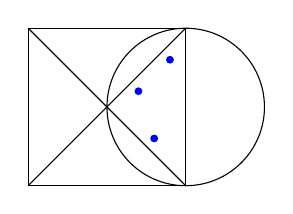
\begin{tikzpicture}[scale=2, rotate=90]
            \draw (0, 0) rectangle (1, 1);
            \draw (0, 0) -- (1, 1);
            \draw (0, 1) -- (1, 0);
            \node[fill=blue, circle, inner sep=1pt] at (0.3, 0.2) {};
            \node[fill=blue, circle, inner sep=1pt] at (0.8, 0.1) {};
            \node[fill=blue, circle, inner sep=1pt] at (0.6, 0.3) {};
            \draw (0.5, 0) circle (0.5);
        \end{tikzpicture}
    \end{center}
    The circumradius of this triangle is $\frac12$.
\end{proof}

\section{Mathematical Induction} \label{sec:induction}
\begin{example}
    Let $f(m)$ be the maximum number of regions into which $m$ lines divide
    the plane.
    \begin{center}
        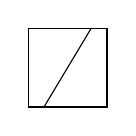
\begin{tikzpicture}
            \draw (0, 0) rectangle (1, 1);
            \draw (0.2, 0) -- (0.8, 1);
        \end{tikzpicture}
        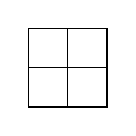
\begin{tikzpicture}
            \draw (0, 0) rectangle (1, 1);
            \draw (0.5, 0) -- (0.5, 1);
            \draw (0, 0.5) -- (1, 0.5);
        \end{tikzpicture}
        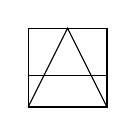
\begin{tikzpicture}
            \draw (0, 0) rectangle (1, 1);
            \draw (0, 0) -- (0.5, 1) -- (1, 0);
            \draw (0, 0.4) -- (1, 0.4);
        \end{tikzpicture}
    \end{center}
    Then $f(m) \le \binom{m}{0} + \binom{m}{1} + \binom{m}{2}$ for all
    $m \ge 0$.
\end{example}
\begin{proof}
    The base case $m = 1$ is true by observation.

    Suppose the statement is true for some $m \ge 1$.
    Then there exists an arrangement $A$ of $m$ lines with $f(n)$ regions.
    Suppose $l$ is the $(m+1)$th line added to $A$, which intersects $k$
    lines.
    Then it divides $k+1$ regions into two, so that the number of regions
    increases by $k+1 \le m+1$.
    Thus \begin{align*}
        f(m+1) &\le f(m) + m + 1 \\
            &\le \binom{m}{0} + \binom{m}{1} + \binom{m}{2} + \binom{m+1}{1} \\
            &= \binom{m+1}{0} + \binom{m+1}{1} + \binom{m+1}{2}. \qedhere
    \end{align*}
\end{proof}

\begin{example}[Wrong]
    All cows are the same colour.
\end{example}
\begin{proof}[``Proof'']
    We rephrase this as follows: for all $n \in \N^*$, all sets of $n$ cows
    are the same colour.

    Trivially true for one cow.
    Suppose it is true for all sets of $n \ge 1$ cows.
    Consider a set of $n+1$ cows.
    Label them $c_1, \dots, c_{n+1}$.
    By the inductive hypothesis, $\set{c_1, c_2, \dots, c_n}$ are the same
    colour.
    Similarly, $\set{c_2, \dots, c_n, c_{n+1}}$ are the same colour.
    Thus $c_1$ and $c_{n+1}$ are the same colour.
    By induction, all cows are the same colour.
\end{proof}
